\chapter{Implementación de intregradores fracionarios}

	\section{¿Qué es una FPAA?}
	Una FPAA  por sus siglas en inglés (Field Programmable Analog Arrays) es un dispositivo analógico equivalente a las FPGA (Field Programmable Garte Arrays). A diferencia de las FPGA que contienen una gran cantidad de módulos y conexiones que permiten configuraciones arbitrarias de lógica combinacional y secuencial, los FPAA generalmente contienen una pequeña cantidad de CABs (Configurable Analog Blocks). Los FPAA dirigidos al diseño analógico estándar generalmente presentan un CAB que contiene un amplificador operacional, un arreglo de capacitores programables, y ya sea un arreglo de resistencias programables para circuitos en tiempo continuo o switches configurables para circuitos de capacitores conmutados.
	Se trabajó con la tarjeta Anadigm QuadApex Develovment Boarsd v2.0 de la empresa Anadigm, la cual contiene 4 FPAAs AN231E04 que pueden conectarse en cadena y es programada mediante el software AnadigmDesigner2 (AD2). El diagrama esquemático de la tarjeta se puede ver en la Figura \ref{fig:esquematico_fpaa} del apéndice.
	
	\section{Características de la tarjeta y requerimientos}
	
		\subsection{Alimentación de la tarjeta}
	
		\subsection{Instalación de drivers}

		\subsection{Jumpers por defecto}

		\subsection{Tamaño variable de cadena de FPAAs}

		\subsection{DIP Switches}
	
		\subsection{Filtros Rauch y buffers de salida}\label{sec:rauch}
	
		\subsection{Circuito de prueba}
		
	\section{AnadigmDesigner2}
	
		\subsection{Comunicación con AD2}\label{sec:comunicacion_con_AD2}

		\subsection{Equivalencia de conexiones en tarjeta y en software}
		
	\begin{table}[!ht]                                      
		\centering   
		\caption{Equivalencias de IOCell en AD2 a físicos pines en tarjeta en FPAA.}                            
		\label{tab:IOresumen}                                        
			\begin{tabular}{ll cc ll cc ll cc ll cc ll}                        
			\hline                                              
			\multicolumn{2}{c}{IOCell 1} &&& \multicolumn{2}{c}{IOCell 2} &&& \multicolumn{2}{c}{IOCell 3}	&&& \multicolumn{2}{c}{IOCell 4}\\            
			\hline                                              
			01	& I1P	&&&	09	& I2P	&&&	11	& I3P	&&&	24	& I4P	\\  
			02	& I1N	&&&	08	& I2N	&&&	12	& I3N	&&&	23	& I4N	\\
			04	& O1P	&&&	06	& 02P	&&&	14	& 03P	&&&	21	& 04P	\\
			03	& O1N	&&&	07	& 02N	&&&	13	& 03N	&&&	22	& 04N	\\
			\hline
				&&&&&&&&&&&&& 	\\                                 
			\end{tabular}
		
			\begin{tabular}{ll cc ll cc ll cc ll cc ll}                        
			\hline                                              
			\multicolumn{2}{c}{IOCell 5} &&& \multicolumn{2}{c}{IOCell 6} &&& \multicolumn{2}{c}{IOCell 7}	\\            
			\hline                                              
			15	& IO5P	&&&	17	& IO6P	&&&	19	& IO7P	\\  
			16	& IO5N	&&&	18	& IO6N	&&&	20	& IO7N	\\
			\hline                                 
			\end{tabular}                                                             
	\end{table}
	
	\section{NI ELVIS II+}

		\subsection{¿Qué es la NI ELVIS II+?}
	El NI Engineering Laboratory Virtual Instrumentation Suite (NI ELVIS) es un dispositivo modular de laboratorio educativo de ingeniería que incluye un osciloscopio, multímetro digital, generador de funciones, fuente de alimentación variable, \textbf{analizador de Bode} y otros instrumentos comunes de laboratorio. Es necesario utilizar una PC en conjunto con la NI ELVIS para acceder a todas sus prestaciones y la comunicación entre las dos se hace vía USB.

		\subsection{Instalación}
		
		\subsection{Puesta en marcha y calibración}
	
		\subsection{Diagramas de Bode}\label{sec:diagrama_de_bode}
	
		\subsection{Ejemplo práctico}
	Como ejemplo consideremos un filtro pasabajas activo el cual posee la siguiente función de transferencia:
	
	\begin{equation}
		T(s) = - \frac{k \omega_{0}}{s + \omega_{0}}
		\label{ec:pasabajas_TF}
	\end{equation}
	donde:
	\begin{equation}
		\omega_{0} = \frac{1}{R_{f} C} \qquad k = \frac{R_{f}}{R_{i}}
	\end{equation}
	si consideramos los valores $R_{f} = R_{i}= 8.2$k$\Omega$ y $C = 1$uF entonces la función de transferencia (\ref{ec:pasabajas_TF}) se reescribe como:
	
	\begin{equation}
		T(s) = - \frac{1.22 \cdot 10^{5}}{s + 1.22 \cdot 10^{5}}
	\end{equation}
	donde $\omega_{0} = 1.22 \cdot 10^{5} $ y $k = 1$. En la Figura \ref{fig:V8_pasabajas_activo} se muestra el diagrama esquemático del filtro pasabajas activo.
	
	\begin{figure}[hbtp]
		\caption{Diagrama esquemático de filtro pasabajas activo.}
		\label{fig:V8_pasabajas_activo}
		\centering
		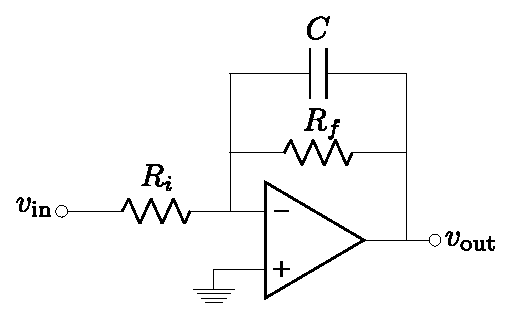
\includegraphics[width = 6.5cm]{V8_pasabajas_activo.eps}
	\end{figure}
	
	Utilizando LTspice se puede hacer la simulación de respuesta en frecuencia del circuito utilizando el modelo spice del amplificador operacional TL081 que se puede encontrar en el siguiente link:
	
	\begin{center}
		\url{http://www.ti.com/lit/zip/sloj069}
	\end{center}
	
	\begin{figure}[!ht]
		\caption{Diagrama de Bode experimental utilizando el NI ELVIS II+.}
		\label{fig:V9_elvis_pasabajas}
		\centering
		\includegraphics[width = 10cm]{V9_elvis_pasabajas.png}
	\end{figure}
	
	\begin{figure}[!ht]
		\caption{Diagramas de Bode comparativos, respuesta ideal, simulación y experimental.}
		\label{fig:V10_bodes_comparativos}
		\centering
		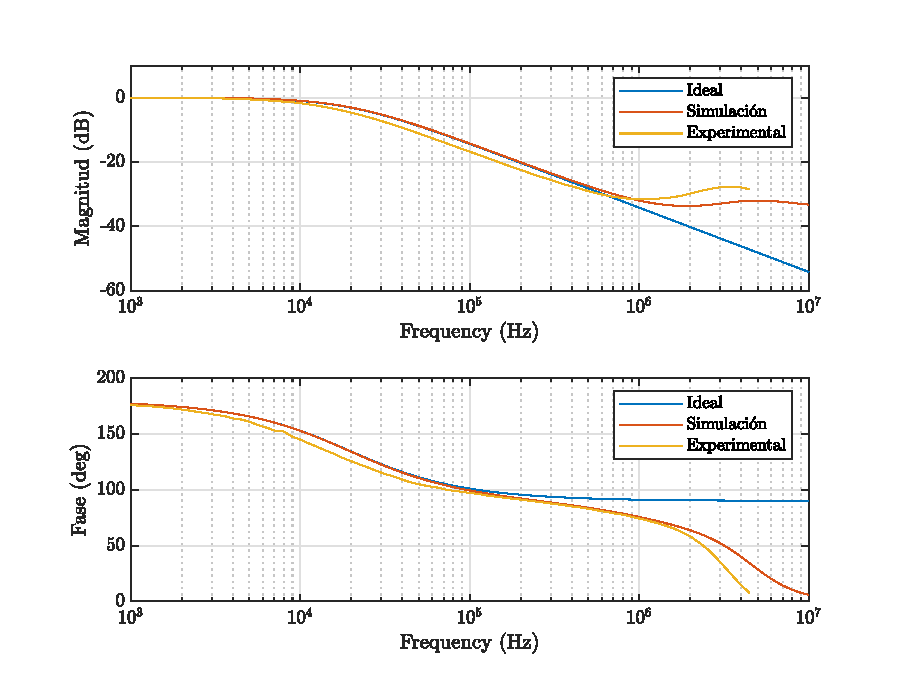
\includegraphics[width = 12cm]{V10_bodes_comparativos.eps}
	\end{figure}
	Los resultados experimentales coinciden casi a la perfección con la simulación . En frecuencias arriba de 1 MHz la respuesta se aleja del comportamiento ideal debido a las limitaciones a altas frecuencias del TL081.
	
	\section{Implementación con aproximación de primer orden}
	
		\subsection{Filtro bilineal configuración polo y cero}

		\subsection{Filtro bilineal configuración pasabajas y pasaaltas}

	
	\section{Implementación con aproximación de segundo}
	
		\subsection{Filtro bicuadrático configuración polo cero}